\documentclass[aspectratio=169, 11pt]{beamer}

% --- Packages & Setup ---
\usepackage[utf8]{inputenc}
\usepackage[T1]{fontenc}
\usepackage{xcolor}
\usepackage{booktabs}
\usepackage{graphicx}
\usepackage{amsmath}
\usepackage{tikz}
\usetikzlibrary{calc, positioning, arrows.meta, shapes.geometric, fit, backgrounds}

\graphicspath{{../}{./}}

% Try loading Open Sans; fallback if missing
\IfFileExists{opensans.sty}{\usepackage[default,scale=0.95]{opensans}}{}

% --- Branding Colors ---
\definecolor{amritaMaroon}{HTML}{A4123F}
\definecolor{inkGrey}{HTML}{3C3C3C}
\definecolor{softGrey}{HTML}{EFEFEF}
\definecolor{lineGrey}{HTML}{B9B9B9}
\definecolor{goodGreen}{HTML}{1A7F43}
\definecolor{warnAmber}{HTML}{9A6700}
\definecolor{coolBlue}{HTML}{2D5BD7}

% --- Theme Setup ---
\usetheme{Madrid}
\usecolortheme[named=amritaMaroon]{structure}
\setbeamertemplate{navigation symbols}{}
\setbeamertemplate{footline}[frame number]
\setbeamertemplate{itemize items}[circle]
\setbeamerfont{frametitle}{size=\large}
\setbeamerfont{framesubtitle}{size=\scriptsize}

% --- Diagram shorthands ---
\tikzset{
  box/.style   = {draw=lineGrey, fill=white, rounded corners=2pt, align=center,
                  font=\scriptsize, inner sep=4pt, minimum height=8mm},
  accent/.style= {draw=amritaMaroon, very thick, fill=amritaMaroon!8},
  blue/.style  = {draw=coolBlue, very thick, fill=coolBlue!8},
  green/.style = {draw=goodGreen, very thick, fill=goodGreen!8},
  amber/.style = {draw=warnAmber, very thick, fill=warnAmber!10},
  zone/.style  = {draw=lineGrey, dashed, rounded corners=4pt, inner sep=7pt},
  fl/.style    = {-{Stealth[length=2mm]}, draw=inkGrey, thick},
  fld/.style   = {-{Stealth[length=2mm]}, draw=lineGrey, thick, dashed},
  lbl/.style   = {font=\tiny\itshape, text=inkGrey, inner sep=1.5pt}
}

% Small helper for status words in tables
\newcommand{\ok}[1]{\textcolor{goodGreen}{\textbf{#1}}}
\newcommand{\pend}[1]{\textcolor{warnAmber}{\textbf{#1}}}
\newcommand{\nope}[1]{\textcolor{amritaMaroon}{\textbf{#1}}}

\begin{document}

% ============================================================
% TITLE
% ============================================================
\begin{frame}
    \begin{tikzpicture}[remember picture,overlay]
        \node[fill=amritaMaroon, text=white, font=\bfseries\footnotesize, anchor=north east,
              rounded corners=2pt, inner sep=5pt]
        at ($(current page.north east) + (-0.2cm,-0.2cm)$)
        {Type 1: Research Project};
    \end{tikzpicture}

    \centering
    \IfFileExists{logo.png}{
\includegraphics[width=2.8cm]{logo.png}\vspace{0.1cm}}{\vspace{0.4cm}}

    {\large \textbf{\textcolor{amritaMaroon}{Porygon: Learning Normal Behaviour\\ Inside Running Containers}}} \\
    \vspace{0.08cm}
    {\scriptsize\itshape Does accounting for how a container is deployed yield a more reliable notion of normal behaviour?} \\
    \vspace{0.12cm}
    {\footnotesize \textbf{23CSE498 -- Project Phase 2 (Panel Review 1)} \quad | \quad \textbf{Team Number: [XX]}} \\
    \vspace{0.15cm}

    \begin{table}
        \centering
        \footnotesize
        \renewcommand{\arraystretch}{1.05}
        \begin{tabular}{|c|c|l|}
            \hline
            \textbf{S.No} & \textbf{Register Number} & \textbf{Student Name} \\
            \hline
            1 & CB.EN.U4CSE23XXX & Anurup R Krishnan \\
            \hline
            2 & CB.EN.U4CSE23XXX & Student Name 2 \\
            \hline
            3 & CB.EN.U4CSE23XXX & Student Name 3 \\
            \hline
            4 & CB.EN.U4CSE23XXX & Student Name 4 \\
            \hline
        \end{tabular}
    \end{table}
    \vspace{0.1cm}

    {\footnotesize Guide: \textbf{Guide Name}, Designation, Department of CSE} \\
    \vspace{0.1cm}
    {\scriptsize \today}
\end{frame}

% ============================================================
% THE PROBLEM
% ============================================================
\section{The Problem}
\begin{frame}{The Problem, in Plain Words}
\framesubtitle{Why watching a container is harder than it sounds}

\begin{columns}[T]
\column{0.52\textwidth}
\small
A \textbf{container} is a packaged application that runs isolated on a server.
Companies run thousands of them.

\medskip
If an attacker gets inside one, they run \textbf{programs} that the application
would never normally run --- a command shell, a download tool, a scanner.

\medskip
So the natural idea is: \emph{learn what programs a container normally runs, then
flag the unusual ones.}

\medskip
\textbf{The difficulty.} Before comparing against ``normal'', one must decide
\emph{which} normal. Grouping unlike containers together makes the comparison
meaningless.

\column{0.46\textwidth}
\centering
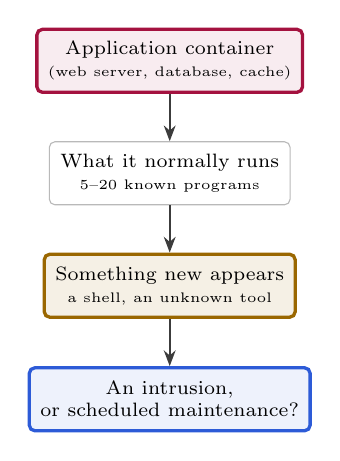
\begin{tikzpicture}[node distance=4mm]
  \node[box, accent, minimum width=30mm] (app) {Application container\\ \tiny(web server, database, cache)};
  \node[box, below=6mm of app, minimum width=30mm] (norm) {What it normally runs\\ \tiny 5--20 known programs};
  \node[box, below=6mm of norm, minimum width=30mm, amber] (odd) {Something new appears\\ \tiny a shell, an unknown tool};
  \node[box, below=6mm of odd, minimum width=34mm, blue] (q) {An intrusion,\\ or scheduled maintenance?};
  \draw[fl] (app) -- (norm);
  \draw[fl] (norm) -- (odd);
  \draw[fl] (odd) -- (q);
\end{tikzpicture}

\smallskip
{\scriptsize Frequently the correct answer is that the evidence is insufficient. The design
reports that state explicitly rather than concealing it.}
\end{columns}
\end{frame}

% ============================================================
% RESEARCH QUESTION
% ============================================================
\begin{frame}{What We Are Actually Asking}
\framesubtitle{The research question, and why it is not obvious}

\begin{columns}[T]
\column{0.45\textwidth}
\footnotesize
Every container image has a \textbf{content fingerprint} --- a code computed from
the exact bytes of the image. Same code, same program; it cannot be faked or
quietly changed.

\medskip
One could group containers by fingerprint and learn a single normal for each.
Is that sufficient?

\medskip
\textbf{Not entirely.} The same image can be \emph{deployed} differently:
another start-up command, user account, permission set or attached folder.
Those differences may change behaviour.

\medskip
\textcolor{amritaMaroon}{\textbf{Our question:}} does adding \emph{how it was
deployed} produce a cleaner normal, or merely divide the data into groups too
small to learn from?

\column{0.53\textwidth}
\centering
\resizebox{\linewidth}{!}{%
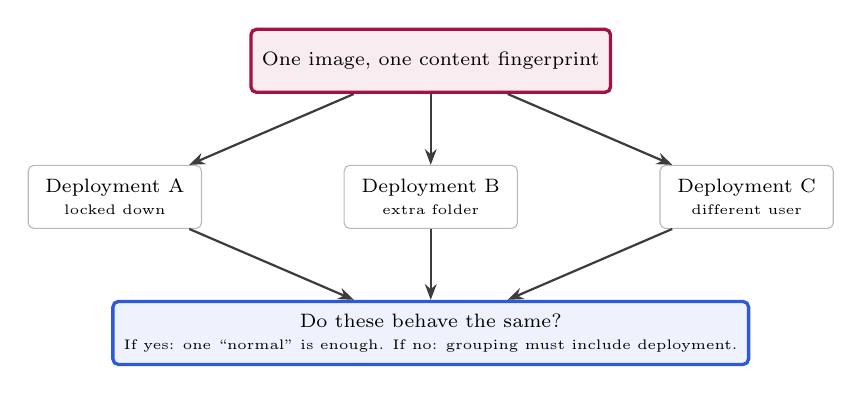
\begin{tikzpicture}[node distance=3mm]
  \node[box, accent, minimum width=42mm] (img) {One image, one content fingerprint};

  \node[box, below left=9mm and 6mm of img, minimum width=22mm] (d1) {Deployment A\\ \tiny locked down};
  \node[box, below=9mm of img, minimum width=22mm] (d2) {Deployment B\\ \tiny extra folder};
  \node[box, below right=9mm and 6mm of img, minimum width=22mm] (d3) {Deployment C\\ \tiny different user};

  \draw[fl] (img) -- (d1);
  \draw[fl] (img) -- (d2);
  \draw[fl] (img) -- (d3);

  \node[box, blue, below=9mm of d2, minimum width=56mm] (q)
    {Do these behave the same?\\ \tiny If yes: one ``normal'' is enough. If no: grouping must include deployment.};
  \draw[fl] (d1) -- (q);
  \draw[fl] (d2) -- (q);
  \draw[fl] (d3) -- (q);
\end{tikzpicture}}

\smallskip
{\scriptsize Four grouping strategies are compared and the measurements decide the outcome.
A result of ``no difference'' is a valid finding, not a failure.}
\end{columns}
\end{frame}

% ============================================================
% RUBRIC 1a: WORKFLOW
% ============================================================
\section{Methodology \& Solution Design}
\begin{frame}{1. Methodology --- How the System Works, End to End}
\framesubtitle{Rubric: Workflow \& Algorithmic Pipeline (5 Marks)}

\centering
\resizebox{\textwidth}{!}{%
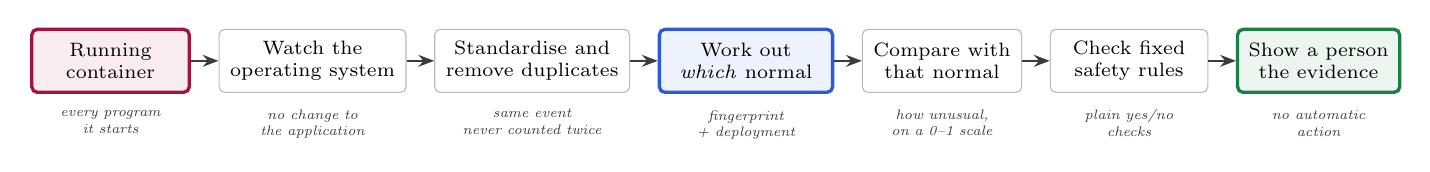
\begin{tikzpicture}[node distance=3.5mm]
  \node[box, accent, minimum width=20mm] (w) {Running\\container};
  \node[box, right=of w, minimum width=21mm] (k) {Watch the\\operating system};
  \node[box, right=of k, minimum width=21mm] (n) {Standardise and\\remove duplicates};
  \node[box, blue, right=of n, minimum width=22mm] (i) {Work out\\\emph{which} normal};
  \node[box, right=of i, minimum width=20mm] (p) {Compare with\\that normal};
  \node[box, right=of p, minimum width=20mm] (r) {Check fixed\\safety rules};
  \node[box, green, right=of r, minimum width=20mm] (h) {Show a person\\the evidence};

  \foreach \a/\b in {w/k, k/n, n/i, i/p, p/r, r/h} \draw[fl] (\a) -- (\b);

  \node[lbl, below=1.5mm of w, text width=20mm, align=center] {every program\\it starts};
  \node[lbl, below=1.5mm of k, text width=21mm, align=center] {no change to\\the application};
  \node[lbl, below=1.5mm of n, text width=21mm, align=center] {same event\\never counted twice};
  \node[lbl, below=1.5mm of i, text width=22mm, align=center] {fingerprint\\+ deployment};
  \node[lbl, below=1.5mm of p, text width=20mm, align=center] {how unusual,\\on a 0--1 scale};
  \node[lbl, below=1.5mm of r, text width=20mm, align=center] {plain yes/no\\checks};
  \node[lbl, below=1.5mm of h, text width=20mm, align=center] {no automatic\\action};
\end{tikzpicture}}

\vspace{4mm}
\begin{columns}[T]
\column{0.48\textwidth}
\footnotesize
\textbf{Two kinds of evidence, deliberately kept separate}
\begin{itemize}\setlength\itemsep{1pt}
  \item \textbf{Statistical:} ``this is rare compared with known-normal runs''
  \item \textbf{Rule-based:} ``a command shell started in a web server''
\end{itemize}
Combining them into a single figure would conceal which of the two applied.

\column{0.48\textwidth}
\footnotesize
\textbf{Deliberately excluded from the design}
\begin{itemize}\setlength\itemsep{1pt}
  \item No automatic shutdown of containers
  \item No opaque machine-learning model
  \item No claim that unusual behaviour indicates an attack
\end{itemize}
\end{columns}
\end{frame}

% ============================================================
% RUBRIC 1b: ARCHITECTURE
% ============================================================
\begin{frame}{1. Methodology --- System Architecture}
\framesubtitle{Rubric: Architecture \& Trust Boundaries (5 Marks)}

\centering
\resizebox{!}{0.62\textheight}{%
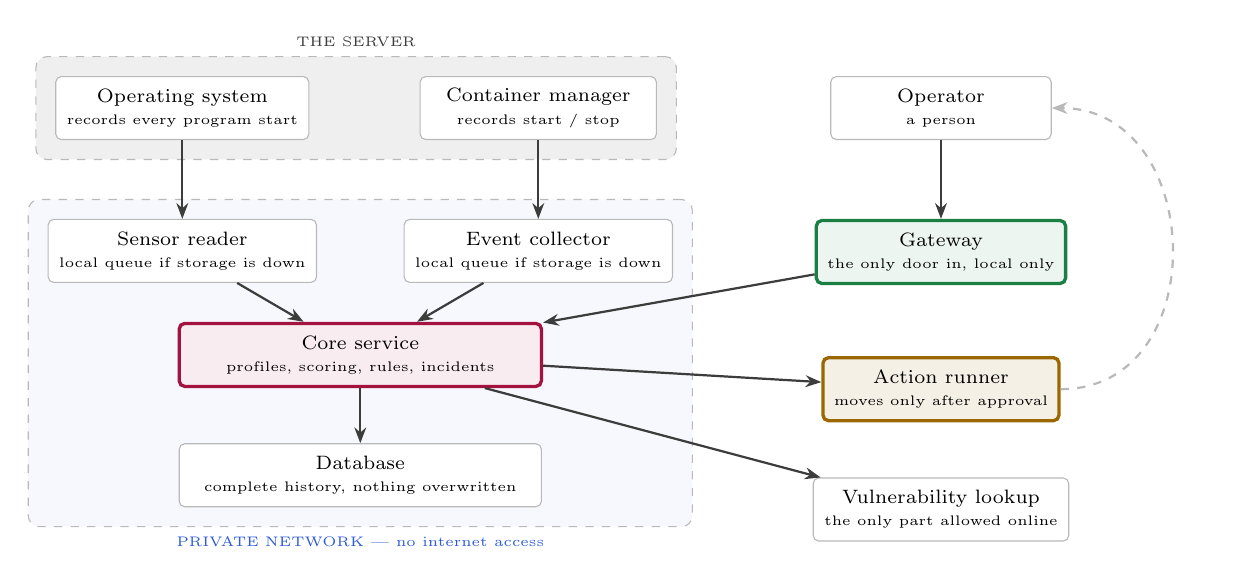
\begin{tikzpicture}[node distance=4mm]

  % --- server zone (top)
  \node[box, minimum width=30mm] (kern) {Operating system\\ \tiny records every program start};
  \node[box, right=14mm of kern, minimum width=30mm] (dock) {Container manager\\ \tiny records start / stop};
  \begin{scope}[on background layer]
    \node[zone, fill=softGrey, fit=(kern)(dock),
          label={[font=\tiny, text=inkGrey]above:THE SERVER}] {};
  \end{scope}

  % --- private zone (middle)
  \node[box, below=10mm of kern, minimum width=30mm] (sensor) {Sensor reader\\ \tiny local queue if storage is down};
  \node[box, below=10mm of dock, minimum width=30mm] (coll) {Event collector\\ \tiny local queue if storage is down};
  \node[box, accent, below=9mm of $(sensor)!0.5!(coll)$, minimum width=46mm]
       (api) {Core service\\ \tiny profiles, scoring, rules, incidents};
  \node[box, below=7mm of api, minimum width=46mm]
       (db) {Database\\ \tiny complete history, nothing overwritten};
  \begin{scope}[on background layer]
    \node[zone, fill=coolBlue!4, fit=(sensor)(coll)(api)(db),
          label={[font=\tiny, text=coolBlue]below:PRIVATE NETWORK --- no internet access}] {};
  \end{scope}

  % --- right column, aligned row-for-row with the left
  \node[box, right=22mm of dock, minimum width=28mm] (op) {Operator\\ \tiny a person};
  \node[box, green, below=10mm of op, minimum width=28mm] (gate) {Gateway\\ \tiny the only door in, local only};
  \node[box, amber, below=9mm of gate, minimum width=28mm] (act) {Action runner\\ \tiny moves only after approval};
  \node[box, below=7mm of act, minimum width=28mm] (scan) {Vulnerability lookup\\ \tiny the only part allowed online};

  \draw[fl] (kern) -- (sensor);
  \draw[fl] (dock) -- (coll);
  \draw[fl] (sensor) -- (api);
  \draw[fl] (coll) -- (api);
  \draw[fl] (api) -- (db);
  \draw[fl] (op) -- (gate);
  \draw[fl] (gate) -- (api);
  \draw[fl] (api) -- (act);
  \draw[fld] (act.east) to[out=0, in=0, looseness=1.4] (op.east);
  \draw[fl] (api) -- (scan);
\end{tikzpicture}}

\vspace{1mm}
{\scriptsize Each part gets the \textbf{least} access it needs. The core service
never reaches the internet; the vulnerability lookup never touches the database;
the action runner only moves when a person has approved.}
\end{frame}

% ============================================================
% RUBRIC 1c: MATHEMATICS
% ============================================================
\begin{frame}{1. Methodology --- The Mathematics}
\framesubtitle{Rubric: Mathematical Model / Formulation (5 Marks)}

\begin{columns}[T]
\column{0.53\textwidth}
\footnotesize
\textbf{Step 1 --- How far has the mix of programs shifted?}\\
Compare the proportions seen now ($q$) with normal ($p$):
\vspace{-1mm}
\[ H(p,q)=\sqrt{\tfrac{1}{2}\textstyle\sum_i\left(\sqrt{p_i}-\sqrt{q_i}\right)^2} \]
\vspace{-3mm}

Always between 0 and 1. Zero means identical.

\medskip
\textbf{Step 2 --- How surprising is the order?}\\
Programs start in habitual sequences. Score each step by how unexpected it is:
\vspace{-1mm}
\[ S=-\tfrac{1}{n}\textstyle\sum \log \hat{P}\!\left(\text{next}\mid\text{current}\right) \]
\vspace{-3mm}

Unobserved pairs retain a small non-zero probability, so no term divides by zero.

\medskip
\textbf{Step 3 --- How much is new?}\\
The proportion of activity whose program never appeared during learning.

\column{0.45\textwidth}
\footnotesize
\textbf{Step 4 --- Combine without arbitrary weights}\\
Each measure is ranked against known-normal runs and the ranks are \textbf{averaged
equally}. A measure that cannot be computed is recorded as unavailable, never
estimated.

\medskip
\textbf{Step 5 --- Express the result on an interpretable scale}\\
Using $n$ complete known-normal runs withheld from learning:
\vspace{-1mm}
\[ p=\frac{1+\#\{\text{normal runs at least this odd}\}}{n+1} \]
\vspace{-3mm}

\smallskip
\textcolor{amritaMaroon}{\textbf{Interpretation:}} approximately one in twenty
normal runs appears this unusual. This is \emph{not} a probability of attack.

\medskip
{\scriptsize\textcolor{warnAmber}{\textbf{Why no tuned weights?}} Earlier fixed
constants ($0.50/0.30/0.20$) had no justification, so the implementation now
accepts none.}
\end{columns}
\end{frame}

% ============================================================
% RUBRIC 1d: METRICS & DATA
% ============================================================
\begin{frame}{1. Methodology --- Data, Splits and Evaluation Metrics}
\framesubtitle{Rubric: Datasets, Preprocessing \& Evaluation Metrics (5 Marks)}

\begin{columns}[T]
\column{0.47\textwidth}
\footnotesize
\textbf{The data is generated, not downloaded.}\\
No public dataset matches this question, so we produce our own under controlled
conditions: three real, widely used server programs, each locked to an exact
image fingerprint.

\smallskip
\begin{tabular}{@{}ll@{}}
\toprule
\textbf{Program} & \textbf{Locked version} \\
\midrule
Web server & nginx 1.26.3 \\
In-memory store & Redis 7.2.7 \\
Database & PostgreSQL 16.6 \\
\bottomrule
\end{tabular}

\smallskip
Each is run idle, under steady load, under bursts, and with deployment changes.
Harmless but unusual activity (backups, restarts, maintenance) is recorded too:
these are the cases that generate false alarms.

\smallskip
\textbf{Splitting rule:} a \emph{whole run} goes to learning, calibration or
testing, never divided. Observations seconds apart are near-duplicates; treating
them as independent would overstate confidence.

\column{0.51\textwidth}
\footnotesize
\textbf{What we will measure}

\begin{tabular}{@{}p{2.6cm}p{4.6cm}@{}}
\toprule
\textbf{Group} & \textbf{Measures} \\
\midrule
Getting it right & false-alarm rate on harmless runs; how many planted events are caught \\
Trustworthy data & events created vs.\ events stored, at every hand-off point \\
Speed & delay from event to stored record (typical, slow, worst) \\
Cost & processor time, memory, disk growth, slowdown of the watched app \\
Honesty of scale & do 95\% of normal runs really score inside the 95\% band? \\
\bottomrule
\end{tabular}

\smallskip
\textcolor{amritaMaroon}{\textbf{Reporting standard:}} every percentage is
published with the counts that produced it. No figure appears without the runs
behind it.
\end{columns}
\end{frame}

% ============================================================
% RUBRIC 2a: STATUS
% ============================================================
\section{Implementation Progress}
\begin{frame}{2. Implementation Progress --- Module Status}
\framesubtitle{Rubric: Core Modules Implemented, Functional \& Integrated (8 Marks)}

\centering
\begin{table}
\scriptsize
\renewcommand{\arraystretch}{1.02}
\begin{tabular}{p{3.3cm} p{6.1cm} c}
\toprule
\textbf{Module} & \textbf{What it does today} & \textbf{Status} \\
\midrule
System-level watcher        & Every program start, in every container   & \ok{Working} \\
Container event collector & Start/stop events; resolves the exact image identity & \ok{Working} \\
Safe delivery             & Local queue; never skips an event it failed to store & \ok{Working} \\
Storage \& history        & 9 schema upgrades; nothing overwritten             & \ok{Working} \\
Deployment fingerprint    & Turns a deployment into one repeatable identity      & \ok{Working} \\
Behaviour profiles        & Builds and versions ``normal''; refuses weak ones     & \ok{Working} \\
Unusualness scoring       & Explainable score with its reasons attached          & \ok{Working} \\
Rule-based evidence       & Fixed checks, incident timeline, human sign-off      & \ok{Working} \\
Approved action runner    & Pause or stop, only after a person approves             & \ok{Working} \\
Vulnerability lookup      & Software inventory per image; known-exploited flags     & \ok{Working} \\
Experiment harness        & Runs real containers; tamper-evident results & \ok{Working} \\
\midrule
Four-way comparison    & The core research comparison                       & \nope{Not started} \\
Result tables, figures & Cannot exist before the study runs                   & \nope{Not started} \\
\bottomrule
\end{tabular}
\end{table}

\vspace{-2mm}
{\scriptsize \textbf{Overall $\approx$65\%} --- platform $\approx$90\% complete,
evaluation $\approx$15\%. The split is reported rather than a single figure.}
\end{frame}

% ============================================================
% RUBRIC 2b: EVIDENCE
% ============================================================
\begin{frame}{2. Implementation Progress --- Evidence of Working Software}
\framesubtitle{Rubric: Functional \& Integrated (8 Marks)}

\begin{columns}[T]
\column{0.44\textwidth}
\footnotesize
\textbf{Size and coverage}

\begin{tabular}{@{}lr@{}}
\toprule
Lines of program code & 17{,}802 \\
Automated tests passing & \ok{156} \\
Service interfaces & 64 \\
Database upgrade steps & 9 \\
Services running together & 8 \\
\bottomrule
\end{tabular}

\medskip
\textbf{Automatic checks, all passing}

\begin{tabular}{@{}p{3.6cm}c@{}}
\toprule
Code \& configuration & \ok{pass} \\
All unit tests & \ok{pass} \\
Live end-to-end run & \ok{pass} \\
Real-container run & \ok{pass} \\
\bottomrule
\end{tabular}

\column{0.53\textwidth}
\footnotesize
\textbf{Measured on real containers (16 runs)}

\begin{tabular}{@{}p{4.3cm}r@{}}
\toprule
Marked test events created & 96 \\
Seen by the system watcher & \ok{96} \\
Stored in the database & \ok{96} \\
Lost & \ok{0} \\
Counted twice & \ok{0} \\
Application requests served & 360/360 \\
Leftover containers after cleanup & \ok{0} \\
\bottomrule
\end{tabular}

\medskip
\textbf{Complete chain proven on real data}
\smallskip

\resizebox{\linewidth}{!}{%
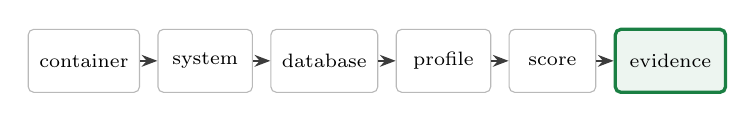
\begin{tikzpicture}[node distance=2.2mm]
  \node[box, minimum width=13mm] (a) {container};
  \node[box, right=of a, minimum width=12mm] (b) {system};
  \node[box, right=of b, minimum width=13mm] (c) {database};
  \node[box, right=of c, minimum width=12mm] (d) {profile};
  \node[box, right=of d, minimum width=11mm] (e) {score};
  \node[box, green, right=of e, minimum width=14mm] (f) {evidence};
  \foreach \x/\y in {a/b,b/c,c/d,d/e,e/f} \draw[fl] (\x) -- (\y);
\end{tikzpicture}}

\smallskip
{\scriptsize From a real database container: 479 recorded program starts became a
profile, a later window scored \emph{normal-looking}, and 72 rule checks matched
without raising a false incident.}
\end{columns}
\end{frame}

% ============================================================
% RUBRIC 2c: SAFETY BEHAVIOUR
% ============================================================
\begin{frame}{2. Implementation Progress --- The Safety Rails Work}
\framesubtitle{Live demonstration: the conditions under which the system declines}

\begin{columns}[T]
\column{0.5\textwidth}
\footnotesize
A system of this kind is only trustworthy if it declines at the correct moments.
Three such refusals can be demonstrated live:

\medskip
\textbf{1. It refuses a weak profile.}\\
Asked to learn ``normal'' from too little data, it stops:\\
{\tiny\ttfamily needed 3 time windows, found 2}

\medskip
\textbf{2. It refuses to evaluate itself on its own training data.}\\
Asked to score a period it already learned from:\\
{\tiny\ttfamily scoring windows must not overlap the training interval}

\medskip
\textbf{3. It refuses an unstable reference.}\\
Asked to use a version label instead of an exact fingerprint:\\
{\tiny\ttfamily refusing a mutable image reference}

\column{0.48\textwidth}
\centering
\resizebox{!}{0.58\textheight}{%
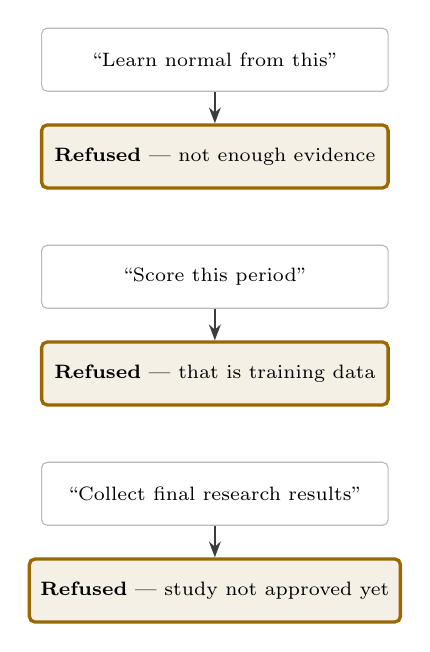
\begin{tikzpicture}[node distance=4mm]
  \node[box, minimum width=44mm] (r1) {``Learn normal from this''};
  \node[box, amber, below=4mm of r1, minimum width=44mm] (x1) {\textbf{Refused} --- not enough evidence};
  \node[box, below=7mm of x1, minimum width=44mm] (r2) {``Score this period''};
  \node[box, amber, below=4mm of r2, minimum width=44mm] (x2) {\textbf{Refused} --- that is training data};
  \node[box, below=7mm of x2, minimum width=44mm] (r3) {``Collect final research results''};
  \node[box, amber, below=4mm of r3, minimum width=44mm] (x3) {\textbf{Refused} --- study not approved yet};
  \draw[fl] (r1) -- (x1); \draw[fl] (r2) -- (x2); \draw[fl] (r3) -- (x3);
\end{tikzpicture}}

\smallskip
{\scriptsize Each refusal is enforced in code and covered by an automated test,
so it cannot be bypassed inadvertently.}
\end{columns}
\end{frame}

% ============================================================
% RUBRIC 3a: DESIGN DECISIONS
% ============================================================
\section{Technical Knowledge}
\begin{frame}{3. Technical Knowledge --- Key Decisions and Why}
\framesubtitle{Rubric: Understanding of Methodology, Implementation \& Design Choices (5 Marks)}

\centering
\begin{table}
\scriptsize
\renewcommand{\arraystretch}{1.18}
\begin{tabular}{p{3.3cm} p{4.4cm} p{4.4cm}}
\toprule
\textbf{Decision} & \textbf{Why} & \textbf{What we rejected} \\
\midrule
Identify images by content fingerprint
& A version label can be pointed at different software tomorrow; a fingerprint cannot
& Grouping by container name or version label \\

Watch at the operating-system level
& Sees every program start without changing the application
& Modifying applications, or trusting logs the attacker can edit \\

Use a maintained sensor
& Equivalent evidence at far lower risk than writing new system-level code
& Building a custom system-level sensor: high effort, wide exposure \\

Combine measures by equal average
& No number we cannot justify to an examiner
& Weights tuned until the results look good \\

Judge against held-back normal runs
& Turns a raw distance into ``how often does normal look this odd?''
& Declaring a threshold and calling it accuracy \\

Split by whole runs
& Snapshots seconds apart are near-copies; reusing them fakes confidence
& Random splitting of time windows \\

A person approves every action
& A false alarm must never take down a healthy service
& Automatic shutdown on a score \\
\bottomrule
\end{tabular}
\end{table}
\end{frame}

% ============================================================
% RUBRIC 3b: TRADE-OFFS
% ============================================================
\begin{frame}{3. Technical Knowledge --- Trade-offs We Accepted}
\framesubtitle{Rubric: Design Choices \& Trade-offs (5 Marks)}

\begin{columns}[T]
\column{0.62\textwidth}
\scriptsize
\begin{tabular}{@{}p{3.5cm}p{4.4cm}@{}}
\toprule
\textbf{Benefit} & \textbf{Cost} \\
\midrule
Strong, cheap signal from program starts & Blind to file access and network destinations \\
Cleaner ``normal'' per deployment & Fewer runs per group; some groups too small to judge \\
No unjustifiable tuned numbers & Almost certainly not the most accurate possible \\
Honest confidence intervals & Need far more runs for the same certainty \\
A fair, interpretable scale & Only valid while the workload does not drift \\
No self-inflicted outages & Slower response to a real attack \\
One language across all services & A known write-speed ceiling, not yet a bottleneck \\
\bottomrule
\end{tabular}

\column{0.36\textwidth}
\footnotesize
\textbf{Edge cases already handled}
\begin{itemize}\setlength\itemsep{1pt}
  \item Storage full $\rightarrow$ queue locally, never skip an event
  \item Sensor restarts $\rightarrow$ counters do not go backwards
  \item Same event twice $\rightarrow$ stored once
  \item Malformed input $\rightarrow$ kept as a short, scrubbed sample
  \item Too little data $\rightarrow$ answer ``insufficient'', never guess
  \item Secret on a command line $\rightarrow$ replaced before storage
\end{itemize}
\end{columns}
\end{frame}

% ============================================================
% RUBRIC 3c: FINDINGS
% ============================================================
\begin{frame}{3. Technical Knowledge --- Early Observations}
\framesubtitle{Rubric: Preliminary Observations (5 Marks) --- measured, not expected}

\begin{columns}[T]
\column{0.49\textwidth}
\footnotesize
\textbf{1. No measured data loss to date.}\\
96 marked events created, 96 observed by the system watcher, 96 stored. Points
that cannot yet be measured are labelled as such, never assumed to be zero.

\medskip
\textbf{2. A defect that only repeated runs could reveal.}\\
The deployment identity accidentally included a name that changes every run, so
the same deployment looked different each time. Left unfixed, every group would
have stayed permanently ``too small to judge'' --- and it would have looked like a
finding rather than a defect.

\medskip
\textbf{3. Serving traffic starts no new programs.}\\
40 web requests and 40 database-cache operations produced \emph{zero} recorded
program starts. The profile therefore describes start-up and maintenance activity, a limitation
stated here rather than left implicit.

\column{0.49\textwidth}
\footnotesize
\textbf{4. The deployment changes we tested made no behavioural difference.}

\smallskip
\begin{tabular}{@{}lccc@{}}
\toprule
\textbf{Program} & \textbf{Variants} & \textbf{Events each} & \textbf{Same?} \\
\midrule
Web server & 3 & 46 / 46 / 46 & \ok{yes} \\
Database & 3 & 166 / 166 / 166 & \ok{yes} \\
Cache & 3 & 33 / 33 / 33 & \ok{yes} \\
\bottomrule
\end{tabular}

\smallskip
Restricting permissions and adding a scratch folder changed the \emph{identity}
but not one program that ran.

\smallskip
\textcolor{amritaMaroon}{\textbf{Why this matters now:}} running the full study
with these settings would have produced a ``no benefit'' answer caused by our own
choice of test conditions --- not by the idea being wrong. We will switch to
deployment changes that actually alter which programs run, \emph{before} the
study is locked.

\smallskip
{\scriptsize Identifying this before the study is locked is the purpose of a
trial run.}
\end{columns}
\end{frame}

% ============================================================
% RUBRIC 3d: LIMITS
% ============================================================
\begin{frame}{3. Technical Knowledge --- What We Do Not Claim}
\framesubtitle{Knowing the limits is part of understanding the method}

\begin{columns}[T]
\column{0.49\textwidth}
\footnotesize
\textbf{Unusual is not the same as malicious.}
\begin{itemize}\setlength\itemsep{1pt}
  \item Unusual but harmless: backups, debugging, restarts, a traffic spike
  \item Harmful but ordinary-looking: an attacker using tools already present
\end{itemize}
We keep the two ideas in separate fields and never merge them into one verdict.

\medskip
\textbf{What the system can miss}
\begin{itemize}\setlength\itemsep{1pt}
  \item Anything that is not a program start
  \item Slow activity spread thinly over time
  \item Behaviour that was already present while learning
  \item Any container whose group has too few examples
\end{itemize}

\column{0.49\textwidth}
\footnotesize
\textbf{Not yet claimed, and why}

\begin{tabular}{@{}p{2.9cm}p{3.4cm}@{}}
\toprule
\textbf{Claim} & \textbf{Blocked by} \\
\midrule
Detection accuracy & final study not run \\
False-alarm rate & final study not run \\
Which grouping wins & the comparison itself \\
Suitable for production & single machine, research scope \\
\bottomrule
\end{tabular}

\medskip
\textbf{Current blockers}
\begin{enumerate}\setlength\itemsep{1pt}\footnotesize
  \item Study design awaiting two independent human reviews --- the code refuses to
        collect final results until then
  \item 65\,GB free disk against 150\,GB needed for the full study
  \item Deployment variants need revising (previous slide)
\end{enumerate}
\end{columns}
\end{frame}

% ============================================================
% ROADMAP
% ============================================================
\begin{frame}{Where This Goes Next}
\framesubtitle{From a working platform to an answered question}

\centering
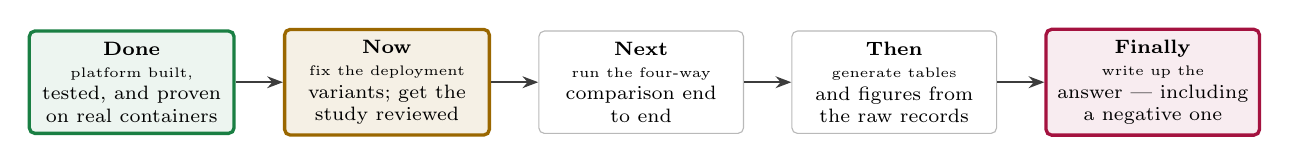
\begin{tikzpicture}[node distance=6mm]
  \node[box, green, minimum width=26mm, minimum height=13mm] (s1)
    {\textbf{Done}\\ \tiny platform built,\\ tested, and proven\\ on real containers};
  \node[box, amber, right=of s1, minimum width=26mm, minimum height=13mm] (s2)
    {\textbf{Now}\\ \tiny fix the deployment\\ variants; get the\\ study reviewed};
  \node[box, right=of s2, minimum width=26mm, minimum height=13mm] (s3)
    {\textbf{Next}\\ \tiny run the four-way\\ comparison end\\ to end};
  \node[box, right=of s3, minimum width=26mm, minimum height=13mm] (s4)
    {\textbf{Then}\\ \tiny generate tables\\ and figures from\\ the raw records};
  \node[box, accent, right=of s4, minimum width=26mm, minimum height=13mm] (s5)
    {\textbf{Finally}\\ \tiny write up the\\ answer --- including\\ a negative one};
  \foreach \a/\b in {s1/s2, s2/s3, s3/s4, s4/s5} \draw[fl] (\a) -- (\b);
\end{tikzpicture}

\vspace{5mm}
\footnotesize
\textbf{The intended contribution} is not container monitoring itself, which is
well-established work. It is a controlled, repeatable comparison of \emph{four
different definitions of what counts as the same thing}, reported faithfully
whichever way the result falls.

\smallskip
Every figure will be traceable to the run that produced it, and every run is
retained so that a reviewer can recompute the tables independently.
\end{frame}

% ============================================================
% RUBRIC 4: ENRICHMENT
% ============================================================
\section{Technical Enrichment}
\begin{frame}{4. Technical Enrichment Activity Choices}
\framesubtitle{Professional Online Certification Details (Individual Mandatory: 10--20 Hours)}
    \begin{itemize}
        \item \textbf{Individual MOOC / Online Certification Selection:}
    \end{itemize}
    \vspace{-0.1cm}
    \begin{table}
        \centering
        \footnotesize
        \renewcommand{\arraystretch}{1.15}
        \begin{tabular}{|c|p{2.8cm}|p{5.0cm}|p{2.3cm}|c|}
            \hline
            \textbf{S.No} & \textbf{Student Name} & \textbf{Chosen MOOC / Course Title} & \textbf{Platform} & \textbf{Hours} \\
            \hline
            1 & Anurup R Krishnan & [e.g. Container Security / Linux Observability] & Coursera & 15 Hrs \\
            \hline
            2 & Student Name 2 & [e.g. Applied Statistics for Experiments] & NPTEL & 20 Hrs \\
            \hline
            3 & Student Name 3 & [e.g. Docker \& Cloud-Native Fundamentals] & edX / Coursera & 12 Hrs \\
            \hline
            4 & Student Name 4 & [e.g. Cloud Security Foundations] & AWS / Google & 16 Hrs \\
            \hline
        \end{tabular}
    \end{table}
    \vspace{0.15cm}
    \begin{itemize}
        \item {\scriptsize \textbf{Requirement:} Each student must complete one approved 10--20 hour online certification from a recognized platform (Coursera, NPTEL, edX, etc.) relevant to the project.}
        \item {\scriptsize \textbf{Note:} course titles above are suggestions aligned to the project's four skill areas --- container internals, operating-system observation, experiment design, and security practice. Replace with the actual enrolled courses and attach completion certificates.}
    \end{itemize}
\end{frame}

% ============================================================
% REFERENCES
% ============================================================
\section{References}
% Self-contained so the deck compiles anywhere. If IEEEtran.bst is installed on
% your machine, delete this frame and use the ref.bib file shipped alongside:
%     \bibliographystyle{IEEEtran}
%     \bibliography{ref}
\begin{frame}[allowframebreaks]{References}
\scriptsize
\begin{thebibliography}{9}

\bibitem{forrest1996}
S.~Forrest, S.~A. Hofmeyr, A.~Somayaji, and T.~A. Longstaff,
``A sense of self for Unix processes,''
in \emph{Proc. IEEE Symp. Security and Privacy}, 1996, pp.~120--128.

\bibitem{hofmeyr1998}
S.~A. Hofmeyr, S.~Forrest, and A.~Somayaji,
``Intrusion detection using sequences of system calls,''
\emph{Journal of Computer Security}, vol.~6, no.~3, pp.~151--180, 1998.

\bibitem{abed2015}
A.~S. Abed, T.~C. Clancy, and D.~S. Levy,
``Applying bag of system calls for anomalous behavior detection of applications
in Linux containers,''
in \emph{Proc. IEEE Globecom Workshops}, 2015, pp.~1--5.

\bibitem{lin1991}
J.~Lin,
``Divergence measures based on the Shannon entropy,''
\emph{IEEE Trans. Information Theory}, vol.~37, no.~1, pp.~145--151, 1991.

\bibitem{vovk2005}
V.~Vovk, A.~Gammerman, and G.~Shafer,
\emph{Algorithmic Learning in a Random World}.
New York, NY, USA: Springer, 2005.

\bibitem{shafer2008}
G.~Shafer and V.~Vovk,
``A tutorial on conformal prediction,''
\emph{Journal of Machine Learning Research}, vol.~9, pp.~371--421, 2008.

\bibitem{gregg2019}
B.~Gregg,
\emph{BPF Performance Tools: Linux System and Application Observability}.
Boston, MA, USA: Addison-Wesley, 2019.

\bibitem{falco}
The Falco Authors,
``Falco: cloud-native runtime security,''
Cloud Native Computing Foundation. [Online]. Available: https://falco.org

\bibitem{ociimage}
Open Container Initiative,
``OCI image format specification.'' [Online].
Available: https://github.com/opencontainers/image-spec

\end{thebibliography}
\end{frame}

% ============================================================
% THANK YOU
% ============================================================
\begin{frame}
    \centering
    {\Huge \textbf{\textcolor{amritaMaroon}{Thank You}}}

    \vspace{6mm}
    {\footnotesize Questions welcome, including those on the limits of what this\\
    system can currently demonstrate.}
\end{frame}

\end{document}
